\documentclass[12pt,a4paper]{article}

% 基础包
\usepackage{geometry}
\usepackage{fancyhdr}
\usepackage{amsmath,amssymb,amsthm}
\usepackage{graphicx}
\usepackage{booktabs}
\usepackage{hyperref}
\usepackage{enumitem}

% 增强数学建模的包
\usepackage{tikz}               % 绘图
\usepackage{pgfplots}           % 绘制高质量图表
\usepackage{algorithm2e}        % 算法伪代码
\usepackage{siunitx}            % 单位处理
\usepackage{multirow}           % 表格增强
\usepackage{xcolor}             % 颜色支持
\usepackage{listings}           % 代码展示
\usepackage{subcaption}         % 子图形
\usepackage{lastpage}
% 添加美化目录的包
\usepackage{tocloft}
\usepackage{titlesec}

% 页面布局
\geometry{margin=1in}
% 修改超链接样式:隐藏颜色
\hypersetup{
  hidelinks=true,
  colorlinks=false,
  pdfborder={0 0 0}
}

% 自定义页眉页脚
\pagestyle{fancy}
\fancyhf{}
\renewcommand{\headrulewidth}{0.5pt}
\fancyhead[L]{\textit{Mathematical Modelling Competition}}
\fancyfoot[C]{page \thepage{} of \pageref{LastPage}}
\fancyhead[R]{\textit{Team\#XXXXX}}

% 代码样式设置
\lstset{
  basicstyle=\small\ttfamily,
  breaklines=true,
  frame=single,
  numbers=left,
  numberstyle=\tiny,
  keywordstyle=\color{blue},
  commentstyle=\color{green!60!black},
  stringstyle=\color{purple}
}

% 美化目录设置
\renewcommand{\cfttoctitlefont}{\Large\bfseries}
\renewcommand{\cftbeforesecskip}{10pt}
\renewcommand{\cftaftertoctitle}{\hfill}
\renewcommand{\cftbeforetoctitleskip}{20pt}
\renewcommand{\cftaftertoctitleskip}{30pt}
\renewcommand{\cftsecfont}{\bfseries}
\renewcommand{\cftsecpagefont}{\bfseries}
\renewcommand{\cftbeforesecskip}{8pt}
\setlength{\cftbeforesubsecskip}{4pt}

% 美化节标题
\titleformat{\section}
  {\normalfont\Large\bfseries}{\thesection}{1em}{}[\titlerule]
\titleformat{\subsection}
  {\normalfont\large\bfseries}{\thesubsection}{1em}{}
\titlespacing*{\section}{0pt}{3.5ex plus 1ex minus .2ex}{2.3ex plus .2ex}
\titlespacing*{\subsection}{0pt}{3.25ex plus 1ex minus .2ex}{1.5ex plus .2ex}

\begin{document}

% Abstract page
\begin{center}
  \begin{minipage}{0.95\textwidth}
    \begin{center}
      \Large\textbf{SUMMARY}
      \vspace{0.5cm}
    \end{center}
    \hrule
    \vspace{0.5cm}
    This paper presents a comprehensive mathematical model to address [problem description]. Through multi-factor analysis, weight generation algorithms, and model evaluation systems, we have established a method for objectively evaluating [subject]. The model considers the influence of time variation on various factors and can be extended to related fields. The effectiveness and practical value of the model have been demonstrated through data validation and sensitivity analysis.
    \vspace{0.5cm}
    \hrule
  \end{minipage}
\end{center}
\newpage

% 目录标题美化
\renewcommand{\contentsname}{\centerline{CONTENTS}}
% Table of contents
\tableofcontents
\newpage

\section{A Problem Introduction}
\subsection{Question Analysis and Restatement}
This section aims to analyze the core elements of the problem and restate it in a form that can be solved using mathematical methods:
\begin{itemize}
  \item Clarify the background and significance of the problem
  \item Determine the boundary conditions and constraints
  \item Transform the practical problem into a mathematical problem
\end{itemize}

Key questions to address:
\begin{enumerate}
  \item What are the essential variables and parameters?
  \item What are the relationships between these variables?
  \item What is the objective function or goal of the problem?
\end{enumerate}

\subsection{Generating Factor Scores}
Before establishing the model, we need to identify and quantify the factors influencing the problem:

\subsubsection{Preliminary Research}
Through literature review, expert consultation, and data analysis, we identify the key factors affecting the problem:
\begin{itemize}
  \item Factor 1: [Description and importance]
  \item Factor 2: [Description and importance]
  \item Factor 3: [Description and importance]
\end{itemize}

\subsubsection{Factor Quantification}
Converting each factor into measurable indicators:

\paragraph{Factor 1 Quantification Method}
\begin{equation}
S_1 = f_1(x_1, x_2, ..., x_n)
\end{equation}
where $x_i$ represents parameters related to Factor 1, and $f_1$ is the quantification function.

\paragraph{Factor 2 Quantification Method}
\begin{equation}
S_2 = f_2(y_1, y_2, ..., y_m)
\end{equation}
where $y_i$ represents parameters related to Factor 2, and $f_2$ is the quantification function.

\subsection{Weight Generation}
Based on the relative importance of factors, we determine the weights using the following method:
\begin{equation}
W_i = \frac{e_i}{\sum_{j=1}^n e_j}
\end{equation}
where $W_i$ is the weight of the $i$-th factor, and $e_i$ is the eigenvalue obtained through analytic hierarchy process or other methods.

\subsubsection{Weight Matrix Assessment and Optimization}
To ensure the rationality of weight allocation, we calculate the consistency ratio:
\begin{equation}
CR = \frac{CI}{RI}
\end{equation}
where $CI$ is the consistency index and $RI$ is the random consistency index. When $CR < 0.1$, the weight allocation is considered logically consistent.

\subsection{Model Evaluation}
\subsubsection{Model Validity Analysis}
We evaluate the validity of the model through the following methods:
\begin{itemize}
  \item Compare model predictions with actual data
  \item Calculate model prediction error and accuracy
  \item Analyze model performance in different scenarios
\end{itemize}

\subsubsection{Case Studies}
Select typical cases for detailed analysis to demonstrate the practical application of the model.

\subsection{A Broader Evaluation}
\subsubsection{Data Distribution of Factors}
Analyze the distribution characteristics of each factor in the sample, draw distribution graphs, and calculate statistical features:
\begin{figure}[htbp]
  \centering
  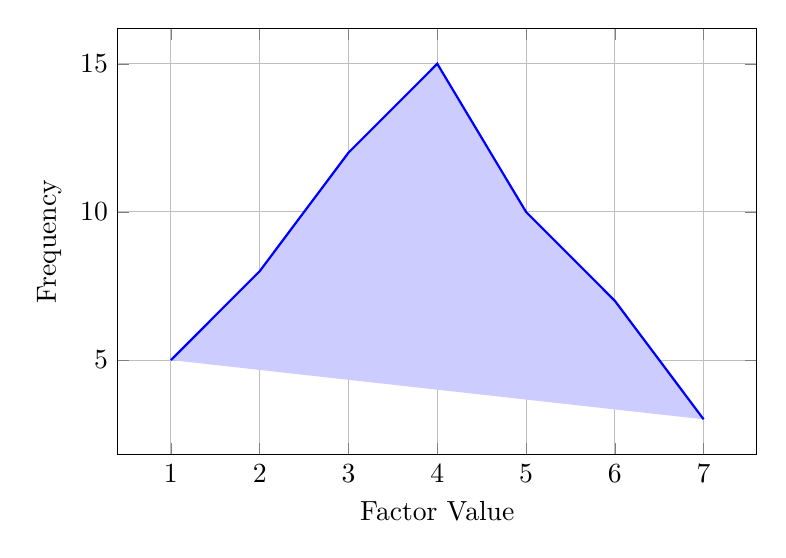
\begin{tikzpicture}
    \begin{axis}[
      width=0.8\textwidth,
      height=7cm,
      xlabel={Factor Value},
      ylabel={Frequency},
      grid=major
    ]
    % Replace with actual data plotting
    \addplot[blue, thick, fill=blue!20] coordinates {
      (1, 5) (2, 8) (3, 12) (4, 15) (5, 10) (6, 7) (7, 3)
    };
    \end{axis}
  \end{tikzpicture}
  \caption{Factor Distribution Diagram}
  \label{fig:factor_distribution}
\end{figure}

\section{Model for Other Applications}
\subsection{Introduction}
Building on the foundation of the basic model, we extend the model to broader application scenarios, considering more variables and conditions.

\subsection{Research on Extended Applications}
To extend the model, additional research is needed:
\begin{itemize}
  \item Special requirements and conditions of related fields
  \item Characteristics and impact of new variables
  \item Existing research achievements and practical experience
\end{itemize}

\subsubsection{Quantification of Additional Factors}
For additional factors in the extended model, we employ similar quantification methods:
\begin{equation}
S_{new} = f_{new}(z_1, z_2, ..., z_k)
\end{equation}
where $z_i$ represents parameters related to the new factor, and $f_{new}$ is the quantification function.

\subsection{Model Evaluation}
Comprehensively evaluate the extended model to ensure its applicability and accuracy:
\begin{itemize}
  \item Verify model performance in new scenarios
  \item Comparative analysis with the original model
  \item Adjust model parameters to optimize performance
\end{itemize}

\subsection{Interaction of Elements}
Study the interaction and influence between multiple elements in the model:
\begin{equation}
I(A, B) = \alpha \cdot f_A + \beta \cdot f_B + \gamma \cdot f_{AB}
\end{equation}
where $I(A, B)$ represents the interaction effect of elements A and B, $f_A$ and $f_B$ represent the independent effects of A and B, $f_{AB}$ represents their interaction effect, and $\alpha$, $\beta$, and $\gamma$ are the corresponding coefficients.

\subsubsection{Quantifying Interaction Effects}
Quantify interaction effects through the following method:
\begin{equation}
f_{AB} = \sum_{i=1}^m \omega_i \cdot c_{AB,i}
\end{equation}
where $\omega_i$ is the weight of the $i$-th interaction indicator, and $c_{AB,i}$ is the interaction score of A and B on this indicator.

\section{Future Considerations}
\subsection{Effect of Time on Factors}
Consider dynamic models that change with time:
\begin{equation}
F_i(t) = F_i(0) + \Delta F_i \cdot t + \varepsilon(t)
\end{equation}
where $F_i(t)$ represents the value of the $i$-th factor at time $t$, $F_i(0)$ is the initial value, $\Delta F_i$ is the rate of change, and $\varepsilon(t)$ is the random fluctuation term.

\begin{figure}[htbp]
  \centering
  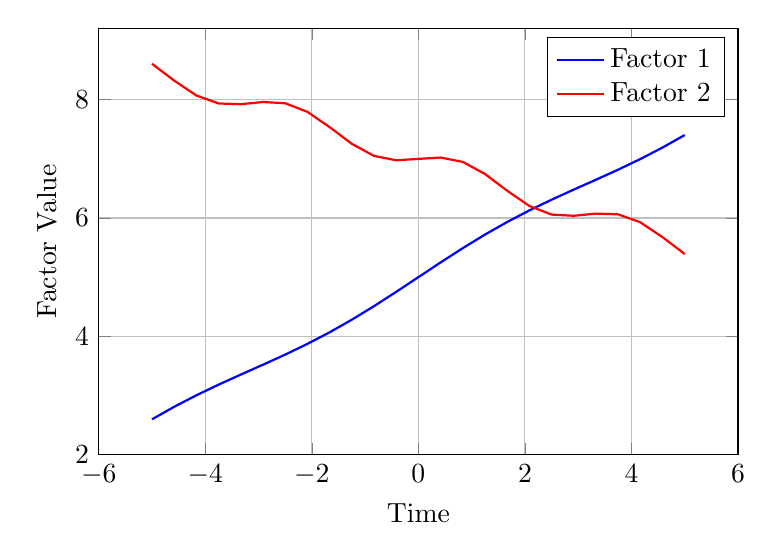
\begin{tikzpicture}
    \begin{axis}[
      width=0.8\textwidth,
      height=7cm,
      xlabel={Time},
      ylabel={Factor Value},
      grid=major
    ]
    % Replace with actual data plotting
    \addplot[blue, thick] {5 + 0.5*x + 0.1*sin(deg(x))};
    \addplot[red, thick] {7 - 0.3*x + 0.2*sin(deg(2*x))};
    \legend{Factor 1, Factor 2}
    \end{axis}
  \end{tikzpicture}
  \caption{Factor Trends Over Time}
  \label{fig:time_trend}
\end{figure}

\section{Conclusion}
\subsection{Model Evaluation}
Summarize the overall performance and applicability of the model:
\begin{itemize}
  \item Accuracy and reliability of the model
  \item Model performance in different scenarios
  \item Fit between model and actual problems
\end{itemize}

\subsection{Strength of Model}
Analyze the main advantages of the model:
\begin{itemize}
  \item Comprehensive consideration of multiple influencing factors
  \item Flexible adaptation to different application scenarios
  \item Good interpretability
  \item High computational efficiency and easy implementation
\end{itemize}

\subsection{Things to Improve}
Identify the limitations of the model and possible future improvements:
\begin{itemize}
  \item Introduction of more fine-grained factors
  \item Improvement of quantification algorithm accuracy
  \item Development of more efficient computation methods
  \item Extension to more application domains
\end{itemize}

% References
\newpage
\begin{thebibliography}{99}
\bibitem{ref1} Author, A. (Year). \textit{Title}. Journal, Volume(Issue), Pages.
\bibitem{ref2} Author, B. (Year). \textit{Title}. Publisher, City.
\bibitem{ref3} Author, C. (Year). \textit{Title}. Conference Name, Pages.
\bibitem{ref4} Author, D. (Year). \textit{Title}. URL, Access Date.
\end{thebibliography}

% Appendices
\newpage
\appendix

\section{Algorithm Implementation}
Provides pseudocode and implementation examples of core algorithms for the model:
\begin{algorithm}[H]
\SetAlgoLined
\KwIn{Input parameter set $P$}
\KwOut{Evaluation result $R$}
Initialize data structures\;
Calculate factor scores $S_i$\;
\For{each factor $i$}{
  Apply weight: $S_i^{weighted} = W_i \times S_i$\;
}
Calculate total score: $S_{total} = \sum_{i} S_i^{weighted}$\;
\If{$S_{total} \geq threshold$}{
  $R \gets$ Condition satisfied\;
}
\Else{
  $R \gets$ Condition not satisfied\;
}
\Return{$R$}
\caption{Model Evaluation Algorithm}
\end{algorithm}

\begin{lstlisting}[language=Python, caption={Model Implementation Example}]
def calculate_model_score(factors, weights):
    # Calculate factor scores
    factor_scores = {}
    for factor_name, factor_data in factors.items():
        factor_scores[factor_name] = quantify_factor(factor_name, factor_data)
    
    # Apply weights
    weighted_scores = {}
    for factor_name in factor_scores:
        weighted_scores[factor_name] = factor_scores[factor_name] * weights[factor_name]
    
    # Calculate total score
    total_score = sum(weighted_scores.values())
    
    # Evaluate result
    result = {
        'total_score': total_score,
        'factor_scores': factor_scores,
        'weighted_scores': weighted_scores,
        'qualified': total_score >= THRESHOLD
    }
    
    return result
\end{lstlisting}



\end{document}